\documentclass[a4paper]{book}
\usepackage[nottoc,numbib]{tocbibind}
\usepackage[english]{babel}
\usepackage[pdftex]{graphics} %enable pdfgraphics support necessary for pdflatex
\usepackage{graphicx}
\usepackage{tikz}
\usepackage[small,bf]{caption}
\usepackage{footmisc}
\usepackage{sidecap}
\usepackage{fancyvrb}
\usepackage{color}
\usepackage{rotating}
\makeatletter
\setlength{\@fptop}{0pt}
\setlength{\@fpsep}{5pt}
\makeatother
\renewcommand{\dotfill}{\leaders\hbox to 5pt{\hss.\hss}\hfill}
\usepackage[hmargin=1.2cm,vmargin=1.5cm]{geometry} %set custom margins
\usepackage{fancyhdr} %enable hyperlinking, highlight page numbers
\usepackage{amsmath}
\usepackage{amssymb}
\numberwithin{equation}{subsection}
\usepackage{amsfonts}
\usepackage{mathrsfs}
\usepackage{tabularx}
\usepackage{lastpage}
\usepackage{subfigure}
\usepackage{multicol}
\usepackage{lipsum}
\usepackage{xspace}
\usepackage{latexsym} 
\usepackage{verbatim}
\usepackage{listings}
\usepackage{color}
\usepackage[usenames,dvipsnames]{xcolor}
\definecolor{listinggray}{gray}{0.9}
\definecolor{lbcolor}{rgb}{0.9,0.9,0.9}
\usepackage{listings}
\usepackage{color}

\definecolor{mygreen}{rgb}{0,0.6,0}
\definecolor{mygray}{rgb}{0.5,0.5,0.5}
\definecolor{mymauve}{rgb}{0.58,0,0.82}

\lstset{ %
   backgroundcolor=\color{white},   % choose the background color; you must add \usepackage{color} or \usepackage{xcolor}
   basicstyle=\footnotesize,        % the size of the fonts that are used for the code
   breakatwhitespace=false,         % sets if automatic breaks should only happen at whitespace
   breaklines=true,                 % sets automatic line breaking
%   captionpos=b,                    % sets the caption-position to bottom
   commentstyle=\color{mygreen},    % comment style
   deletekeywords={...},            % if you want to delete keywords from the given language
   escapeinside={\%*}{*)},          % if you want to add LaTeX within your code
   extendedchars=true,              % lets you use non-ASCII characters; for 8-bits encodings only, does not work with UTF-8
   frame=single,                    % adds a frame around the code
   keepspaces=true,                 % keeps spaces in text, useful for keeping indentation of code (possibly needs columns=flexible)
   keywordstyle=\color{blue},       % keyword style
   language=Octave,                 % the language of the code
   morekeywords={*,...},            % if you want to add more keywords to the set
   numbers=left,                    % where to put the line-numbers; possible values are (none, left, right)
   numbersep=5pt,                   % how far the line-numbers are from the code
   numberstyle=\tiny\color{mygray}, % the style that is used for the line-numbers
   rulecolor=\color{black},         % if not set, the frame-color may be changed on line-breaks within not-black text (e.g. comments (green here))
   showspaces=false,                % show spaces everywhere adding particular underscores; it overrides 'showstringspaces'
   showstringspaces=false,          % underline spaces within strings only
   showtabs=false,                  % show tabs within strings adding particular underscores
   stepnumber=1,                    % the step between two line-numbers. If it's 1, each line will be numbered
   stringstyle=\color{mymauve},     % string literal style
   tabsize=2,                       % sets default tabsize to 2 spaces
%   title=\lstname                   % show the filename of files included with \lstinputlisting; also try caption instead of title
}
% tweak the the style a little bit
\lstdefinestyle{customc}{
%   belowcaptionskip=1\baselineskip,
   breaklines=true,
   frame=single,
   xleftmargin=\parindent,
   language=C++,
%   showstringspaces=false,
   basicstyle=\footnotesize\ttfamily,
   keywordstyle=\bfseries\color{green!40!black},
   commentstyle=\itshape\color{mygray},
   identifierstyle=\color{blue},
   stringstyle=\color{orange},
   framexleftmargin=5mm,
}

\lstset{escapechar=@,style=customc}
\usepackage[sort&compress,numbers]{natbib}

\pagestyle{fancy} %enable custom headeres
\fancyhead{}
\fancyfoot{} %clear predefined headers, then create your own:
\lhead{\footnotesize AliROOT Flow Package manual and documentation}
\rhead{\footnotesize The FLOW team}
\rfoot{\footnotesize Page \thepage\ of \pageref{LastPage}}
\lfoot{\footnotesize \rightmark}
\usepackage[bookmarks=true,
            bookmarksopen=true, 
            bookmarksnumbered=true, pdftex,
            hyperindex=true,linktocpage]{hyperref}
\hypersetup{
    bookmarks=true,         % show bookmarks bar?
    unicode=false,          % non-Latin characters in Acrobat’s bookmarks
    pdftoolbar=true,        % show Acrobat’s toolbar?
    pdfmenubar=true,        % show Acrobat’s menu?
    pdffitwindow=false,     % window fit to page when opened
    pdfstartview={FitH},    % fits the width of the page to the window
    pdftitle={AliROOT Flow Package manual and documentation},    % title
    pdfauthor={Redmer Alexander Bertens},     % author
    pdfsubject={AliROOT Flow Package manual and documentation},   % subject of the document
    pdfcreator={Redmer Alexander Bertens},   % creator of the document
    pdfproducer={Redmer Alexander Bertens}, % producer of the document
    pdfkeywords={ALICE} {AliROOT} {ROOT} {manual} {flow} {package} {software}, % list of keywords
    pdfnewwindow=true,      % links in new window
    colorlinks=true,       % false: boxed links; true: colored links
    linkcolor=blue,          % color of internal links
    citecolor=green,        % color of links to bibliography
    filecolor=blue,      % color of file links
    urlcolor=blue           % color of external links
}
\usepackage{lineno}
\usepackage{makeidx}
\makeindex

\sloppy
\fancypagestyle{plain}
 {
 \fancyhead{}
 \fancyfoot{}
 } % clear header and footer of plain page because of ToC

 % tikxstyle for integration of tikz graphics
\tikzstyle{every node}=[font=\tiny]
\tikzstyle{decision} = [rectangle, draw, fill=yellow!20, 
    rounded corners, minimum height=1.5em, minimum width=2.5em, inner sep=3pt]
\tikzstyle{decision2} = [rectangle, draw, fill=red!20, 
    rounded corners, minimum height=1.5em, minimum width=2.5em, inner sep=3pt]
\tikzstyle{decision3} = [rectangle, draw, fill=green!20, 
    rounded corners, minimum height=1.5em, minimum width=2.5em, inner sep=3pt]
\tikzstyle{block} = [rectangle, draw, fill=blue!20, 
    rounded corners, minimum height=1.5em, minimum width=2.5em, inner sep=3pt]
\tikzstyle{line} = [draw, -latex']
\tikzstyle{cloud} = [draw, ellipse,fill=red!20, 
    minimum height=2em]
\tikzstyle{sdecision} = [rectangle, draw, fill=yellow!20, 
    rounded corners, minimum height=1.5em, minimum width=2.5em, inner sep=3pt]
\tikzstyle{sblock} = [rectangle, draw, fill=blue!20, 
    rounded corners, minimum height=1.5em, minimum width=2.5em, inner sep=3pt]
\tikzstyle{scloud} = [draw, ellipse,fill=red!20, 
    minimum height=2em]
\tikzstyle{ycloud} = [draw, ellipse,fill=yellow!20, 
    minimum height=2em]

\renewcommand{\thefootnote}{\fnsymbol{footnote}}
\frontmatter

\linenumbers
\begin{document}

\noindent
\begin{center}
	\vspace*{1.5cm}
	{\LARGE \bf The FLOW Analysis Package}\\
		
	\vspace{1.5cm}
	\begin{figure}[hbt]
		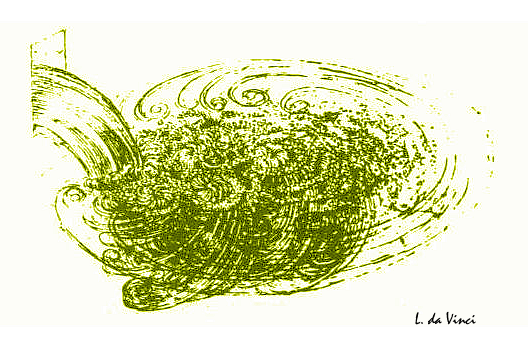
\includegraphics[width=1.\textwidth]{figs/daVinci.png}
	\end{figure}
		
	\vspace{1.5cm}
	\noindent
	{\large \bf a short writeup}\\
	\today\\
\end{center}
\vfill
\noindent
Various authors, edited by Redmer Alexander Bertens (\texttt{rbertens@cern.ch})

\clearpage
\thispagestyle{empty}
\pagenumbering{roman}
\tableofcontents
\renewcommand{\thefootnote}{\alph{footnote}}
\mainmatter
\chapter{Introduction}
The intro to everything.
%-----------------------------------------------------------------------
\chapter{A Quick Start}
\section{The flow package}
\label{quickstart}
The \texttt{ALICE flow package}\index{flow package}\index{ALICE flow package|see{flow package}}\footnote{The \texttt{ALICE} flow package is part of \texttt{AliROOT}\index{AliROOT}, the ALICE extension of the \texttt{ROOT} framework, which can be obtained from \href{http://git.cern.ch/pub/AliRoot}{http://git.cern.ch/pub/AliRoot}. The flow package itself is located in the folder \texttt{\$ALICE\_ROOT/PWG/FLOW/}, where \texttt{\$ALICE\_ROOT} refers to the source directory of \texttt{AliROOT}.} 
contains most known flow analysis methods.  In this chapter we give a few examples how to setup an
analysis for the most common cases. The chapters that follow provide more detailed information on the structure of the code 
and settings of the various flow methods. 
This write-up is however not a complete listing of the methods, for this the reader is referred to the header files.
 
\section{On the fly - getting started on a Toy MC}
To get started with the \texttt{flow package} we begin by generating a few simple Toy Monte Carlo events and performing a flow analysis on these simulated events. The steps which will be followed will be the same as when performing an analysis on data: 
\begin{enumerate}
\item Prepare your \texttt{(Ali)ROOT} session by loaded the necessary libraries
\item Create the analysis method objects
\item Initialize the methods (which creates their histograms)
\item Define track cuts
\item Create flow events, which is a container class holding all necessary information (e.g. tracks) for the flow analysis of an event (collision) and actually do the analysis
\item Finish the analysis, which will calculate the final $v_n$ values
\item Write the results to an output file
\end{enumerate}
In this Monte Carlo exercise, the flow event class will not receive data from a detector (e.g. an \texttt{NTuple}) , but instead generate toy events itself. 

The macro \texttt{runFlowOnTheFlyExample.C}\index{On the fly}\index{runFlowOnTheFlyExample.C}\footnote{In aliroot, this macro can be found at \\ \texttt{\$ALICE\_ROOT/PWGCF/FLOW/Documentation/examples/runFlowOnTheFlyExample}} is a basic example of how the flow package works. 
In this section we explain the main pieces of that macro.
\begin{enumerate}
	\item To use the flow code the flow library needs to be loaded. In\index{libraries, AliROOT} \texttt{AliROOT}:
	\begin{lstlisting}
gSystem->Load("libPWGflowBase");\end{lstlisting}
	In \texttt{root} additional libraries need to be loaded\index{libraries, ROOT}: 
	\begin{lstlisting}
gSystem->Load("libGeom");
gSystem->Load("libVMC");
gSystem->Load("libXMLIO");
gSystem->Load("libPhysics");
gSystem->Load("libPWGflowBase");\end{lstlisting}
	\item We need to instantiate the flow analysis methods which we want to use. In this example we will
	instantiate two methods: the first which calculates the flow versus the reaction plane of the Monte Carlo, which is our reference value\index{reference value}\index{Monte Carlo Event Plane} (see section \ref{MC}), and second the so called Q-cumulant method (see section \ref{qvc}).
	\begin{lstlisting}
AliFlowAnalysisWithMCEventPlane *mcep = new AliFlowAnalysisWithMCEventPlane();
AliFlowAnalysisWithQCumulants *qc = new AliFlowAnalysisWithQCumulants();\end{lstlisting}
	\item Each of the methods needs to initialize\index{initialize methods} (e.g. to define the histograms): 
	\begin{lstlisting}
mcep->Init(); 
qc->Init();\end{lstlisting}
	\item To define the particles we are going to use as Reference Particles\index{reference particles} \index{RP|see{reference particles}} (RP's, particles 
	used for the {\bf Q} vector) and the Particles Of Interest\index{particles of interest} \index{POI|see{particles of interest}} (POI's, the particles of which 
	we calculate the differential flow) we have to define two track cut objects\index{track cut object, simple}:
	\begin{lstlisting}
AliFlowTrackSimpleCuts *cutsRP = new AliFlowTrackSimpleCuts();
AliFlowTrackSimpleCuts *cutsPOI = new AliFlowTrackSimpleCuts();
cutsPOI->SetPtMin(0.2);
cutsPOI->SetPtMax(2.0);	\end{lstlisting}
	\item Now we are ready to start the analysis. For a quick start we make an event on the fly, tag the reference particles and particles of interest  and pass it to the two flow methods. 
	
	We do this in an event loop. First define the number of events that need to be created, their multiplicity, and a value $v_2$ value, which can either be supplied as a fixed number (no $p_t$ dependence) of a function (to generate $p_t$ differential flow\footnote{The on the fly event generator is not limited to the generation of the second harmonic $v_2$, but to get started, this is a nice example}
	
	\begin{lstlisting}
	Int_t nEvents = 1000;	// generate 1000 events
	Int_t mult = 2000;		// use track multiplicity of 2000
	Double_t v2 = .05;		// 5 pct integrated flow
	// or sample differential flow
	TF1* diffv2 = new TF1("diffv2", "((x<1.)*(0.1/1.)*x+(x>=1.)*0.1)", 0., 20.); \end{lstlisting}
	
Now we have all the ingredients to our first flow analysis	
	
	\begin{lstlisting}
// make an event with mult particles 
AliFlowEventSimple* event = new AliFlowEventSimple(mult,AliFlowEventSimple::kGenerate);
// modify the tracks adding the flow value v2
event->AddV2(diffv2);
for(Int_t i=0; i<nEvts; i++) { 
      // select the particles for the reference flow
      event->TagRP(cutsRP);
      // select the particles for differential flow
      event->TagPOI(cutsPOI);
      // do flow analysis with various methods:
      mcep->Make(event);
      qc->Make(event);
      // reset the event so we can re-use the allocated memory
      event->ClearFast();
      // fill the event with a fresh set of tracks
      event->Generate(mult);
} \end{lstlisting}
	\item To fill the histograms which contain the final results we have to call Finish for each method:
	\begin{lstlisting}
mcep->Finish(); 
qc->Finish(); \end{lstlisting}
	\item This concludes the analysis and now we can write the results into a file. Two options for writing the input to a file are available: 
     \begin{itemize}
     \item Create a new output file and write the output to this file
     \begin{lstlisting}
TFile *outputFile = new TFile("outputMCEPanalysis.root","RECREATE");
mcep->WriteHistograms();
TFile *outputFile = new TFile("outputQCanalysis.root","RECREATE");
qc->WriteHistograms();
\end{lstlisting}

Please note that this will create a new output file, and overwrite any existing filse called \texttt{AnalysisResults.root}.

\item  To write the output of multiple analyses into subdirectories of one file, one can do the following:
\begin{lstlisting}
TFile *outputFile = new TFile("AnalysisResults.root","RECREATE");
TDirectoryFile* dirQC = new TDiretoryFile("outputQCanalysis", "outputQCanalysis");
qc->WriteHistograms(dirQC);
TDirectoryFile* dirMCEP = new TDiretoryFile("outputMCEPanalysis", "outputMCEPanalysis");
mcep->WriteHistograms(dirMCEP);
\end{lstlisting}


Note that \texttt{AnalysisResults.root} \index{AnalysisResults.root} is the default name given to analyses in \texttt{AliROOT}. Many macros in \texttt{AliROOT} will expect a file \texttt{AnalyisResults.root} as input, so for most users it will be convenient to follow this convention.

When done with running the analysis, do not forget to write the file to disk by calling
\begin{lstlisting}
TFile::Close();	// write the buffered file to disk \end{lstlisting}
\end{enumerate}

\section{What is in the output file ?}
\index{output file} Now we have written the results into a file, but what is in there? 

Although the output of different flow analysis techniques might differ slightly as a result of their different approaches at estimating $v_2$, the output files containers are always built in a similar way. 

\subsection{AliFlowCommonHists - Output objects}
Objects of two types are stored in the output of the flow analysis\footnote{Make sure that \texttt{libPWGflowBase.so} is loaded in your \texttt{(Ali)ROOT} session, otherwise these objects will be unknown.}
\begin{enumerate}
\item \texttt{AliFlowCommonHist}, which is a class that contains common histograms for the flow analysis (e.g. QA histograms and histograms that contain the analysis flags which were used). Depending on the type of flow analysis that was used, this object contains histograms from the following list:
\begin{lstlisting}
  Bool_t    fBookOnlyBasic;       // book and fill only control histos needed for all methods
  TH1F*     fHistMultRP;          // multiplicity for RP selection
  TH1F*     fHistMultPOI;         // multiplicity for POI selection
  TH2F*     fHistMultPOIvsRP;     // multiplicity for POI versus RP
  TH1F*     fHistPtRP;            // pt distribution for RP selection
  TH1F*     fHistPtPOI;           // pt distribution for POI selection
  TH1F*     fHistPtSub0;          // pt distribution for subevent 0
  TH1F*     fHistPtSub1;          // pt distribution for subevent 1
  TH1F*     fHistPhiRP;           // phi distribution for RP selection
  TH1F*     fHistPhiPOI;          // phi distribution for POI selection
  TH1F*     fHistPhiSub0;         // phi distribution for subevent 0
  TH1F*     fHistPhiSub1;         // phi distribution for subevent 1
  TH1F*     fHistEtaRP;           // eta distribution for RP selection
  TH1F*     fHistEtaPOI;          // eta distribution for POI selection
  TH1F*     fHistEtaSub0;         // eta distribution for subevent 0
  TH1F*     fHistEtaSub1;         // eta distribution for subevent 1
  TH2F*     fHistPhiEtaRP;        // eta vs phi for RP selection
  TH2F*     fHistPhiEtaPOI;       // eta vs phi for POI selection
  TProfile* fHistProMeanPtperBin; // mean pt for each pt bin (for POI selection)
  TH2F*     fHistWeightvsPhi;     // particle weight vs particle phi
  TH1F*     fHistQ;               // Qvector distribution
  TH1F*     fHistAngleQ;          // distribution of angle of Q vector
  TH1F*     fHistAngleQSub0;      // distribution of angle of subevent 0 Q vector
  TH1F*     fHistAngleQSub1;      // distribution of angle of subevent 1 Q vector
  TProfile* fHarmonic;            // harmonic 
  TProfile* fRefMultVsNoOfRPs;    // <reference multiplicity> versus # of RPs
  TH1F*     fHistRefMult;         // reference multiplicity distribution
  TH2F*     fHistMassPOI;         // mass distribution for POI selection \end{lstlisting}
  This information is from the header file of the AliFlowCommonHist object\footnote{The headers of both output objects can be found in \texttt{\$ALICE\_ROOT/PWG/FLOW/Base/}.}
  \item \texttt{AliFlowCommonHistResults} is an object designed to hold the results of the flow analysis. The possible histograms stored in this object are
  \begin{lstlisting}
  TH1D* fHistIntFlow; // reference flow
  TH1D* fHistChi;     // resolution
  // RP = Reference Particles:  
  TH1D* fHistIntFlowRP;     // integrated flow of RPs
  TH1D* fHistDiffFlowPtRP;  // differential flow (Pt) of RPs
  TH1D* fHistDiffFlowEtaRP; // differential flow (Eta) of RPs
  // POI = Particles Of Interest:
  TH1D* fHistIntFlowPOI;     // integrated flow of POIs
  TH1D* fHistDiffFlowPtPOI;  // differential flow (Pt) of POIs
  TH1D* fHistDiffFlowEtaPOI; // differential flow (Eta) of POIs \end{lstlisting}
  
  \end{enumerate}
  The titles of the histograms in the output object differ from the names of the pointers given in the two lists printed above, but the lists give an overview of what is available; the easiest way however of getting acquainted with where to find histograms in the output is browsing them in \texttt{ROOT's TBrowser} (see figure \ref{fig:browserExample}).
  \begin{lstlisting}
  new TBrowser(); \end{lstlisting}
\begin{SCfigure}
 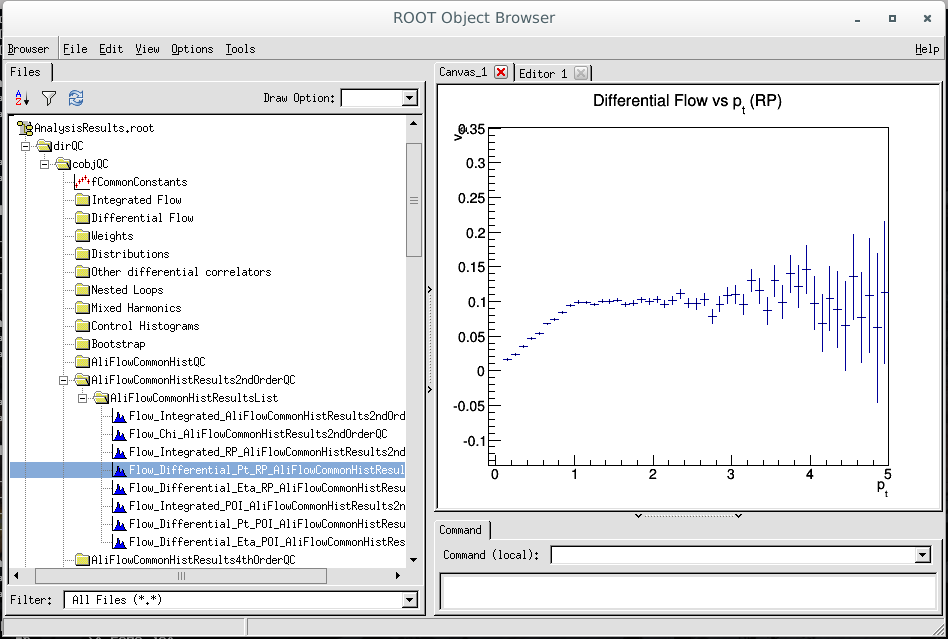
\includegraphics[width=0.70\textwidth]{figs/browserExample.png}
 \caption[TBrowser with output file]{Example of output file opened in a TBrowser, results of differential $v_2$ analysis with second order Q-cumulant analysis are shown.}
 \label{fig:browserExample}
\end{SCfigure}
Analysis specific outputs will be discussed in later sections. 


\subsubsection{Comparing flow results}
A convenient way of comparing the results of the different flow analysis strategies that have been used is invoking the macro \texttt{compareFlowResults.C}\footnote{\texttt{\$ALICE\_ROOT/PWGCF/FLOW/macros/compareFlowResults.C}}.  This macro will read the analysis output file \texttt{AnalysisResults.root}, extract the requested results from it and plot them. For a full overview of what can be done with the macro, the reader is referred to the macro itself and its ample documentation. To run the macro on the dataset that we have just generated, simply do
\begin{lstlisting}
.L compareFlowResults.C
compareFlowResults(TSring(""))	// the empty suffix indicates on the fly events \end{lstlisting}

\begin{SCfigure}
 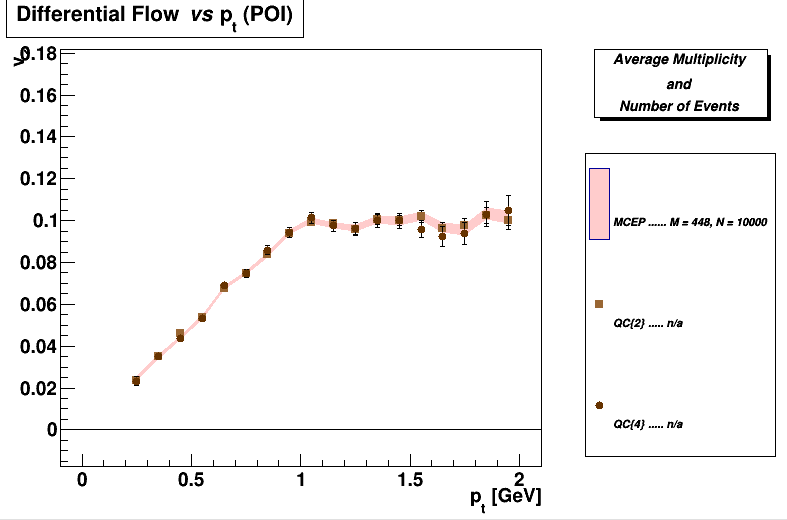
\includegraphics[width=0.70\textwidth]{figs/compareFlowResults.png}
 \caption[Comparing on the fly flow results]{Example of inspecting the output file of the on the fly analysis with the \texttt{compareFlowResults.C macro}.}
 \label{fig:browserExample}
\end{SCfigure}


\subsection{AliFlowCommonConstants - The Common Constants class}
All flow analysis use a common output container to store their histograms. To set the configuration for the histograms in these containers - e.g. the $p_t$ ranges of histograms, the number of bins, etc, etc - all flow analysis methods initialize their output containers using variables from a global instance of the \texttt{AliFlowCommonConstants}\index{AliFlowCommonConstants} class. This global object, which can be obtained via the a static function
\begin{lstlisting}
static AliFlowCommonConstants* GetMaster(); \end{lstlisting} 
can be tuned to the  user's liking by requesting a pointer to it via the static access method, and using the available setter functions, e.g. the following
\begin{lstlisting}
AliFlowCommonConstants* cc = AliFlowCommonConstants::GetMaster();
cc->SetNbinsPt(10);
cc->SetPtMin(0);
cc->SetPtMax(10); \end{lstlisting}
will result in an analysis which is performed in 10 $p_t$ bins of 1 GeV/$c$ width. For a full overview of the available common constants the user is referred to the class header\footnote{\texttt{\$ALICE\_ROOT/PWG/FLOW/Base/AliFlowCommonConstants.h}}.


\subsection{redoFinish.C}
\index{redoFinish.C} When analysis is run in parallel, resulting in large, merged files (e.g. when running on \texttt{GRID}) the output of the flow analysis tasks in \texttt{AnalysisResults.root} is typically wrong, as merging files via \texttt{ROOT's} \texttt{TFileMerger} will trivially sum up results in all histograms. 

The \texttt{redoFinish.C}\footnote{\texttt{\$ALICE\_ROOT/PWGCF/FLOW/macros/refoFinish.C}} macro re-evaluates all output that cannot trivially be merged. To use \texttt{redoFinish.C}, make sure your analysis output file is called \texttt{mergedAnalysisResults.root} and simply run the macro
\begin{lstlisting}
.L redoFinish.C
redoFinish(); \end{lstlisting}
\texttt{redoFinish.C} will produce a new \texttt{AnalysisResults.root} file with the corrected results by calling the \texttt{::Finish()} function on all known output structures in the \texttt{mergedAnalysisResults.root} file. Additionally \texttt{redoFinish.C} can be used to repeat the call to \texttt{::Finish()} with different settings, which might alter the outcome of the flow analysis (e.g. use a different strategy to correct for non-uniform acceptance). This will be explained in more detail in the following sections. 

\section{Getting started on Data}

The macro \texttt{Documentation/examples/runFlowReaderExample.C} \index{runFlowReaderExample.C}is an example how to setup a flow analysis if the events are already generated and
for example are stored in ntuples.
 
\section{A simple flow analysis in ALICE using Tasks}
The macro \texttt{Documentation/examples/runFlowTaskExample.C} \index{runFlowTaskExample.C}is an example how to setup a flow analysis using the full \texttt{ALICE} Analysis Framework.


\chapter{The Program}
The basic idea behind the flow package is that from whatever input you have, a \emph{flow event} is constructed, which is then passed to one or more flow analysis methods (e.g. the scalar product method or Q-cumulant method). The flow event is a collection of \emph{flow tracks}, which are simple objects carrying only the kinematic information that is necessary to do flow analysis. By setting up the flow package in this way, the flow analysis methods can analyze input from various sources, be it ALICE data, Monte Carlo events, STAR data, etc, etc, as long as the flow event is properly filled. This might all sound a bit abstract at this point; this chapter however will explain all details and relevant classes in detail. For those who are impatient and prefer seeing the flow package in action, section \ref{sec:example} gives a step-by-step example of doing a $\pi^{\pm}$ $v_2$ analysis in the \texttt{AliROOT} analysis framework. 

\section{Overview}
\begin{figure}
\begin{center}
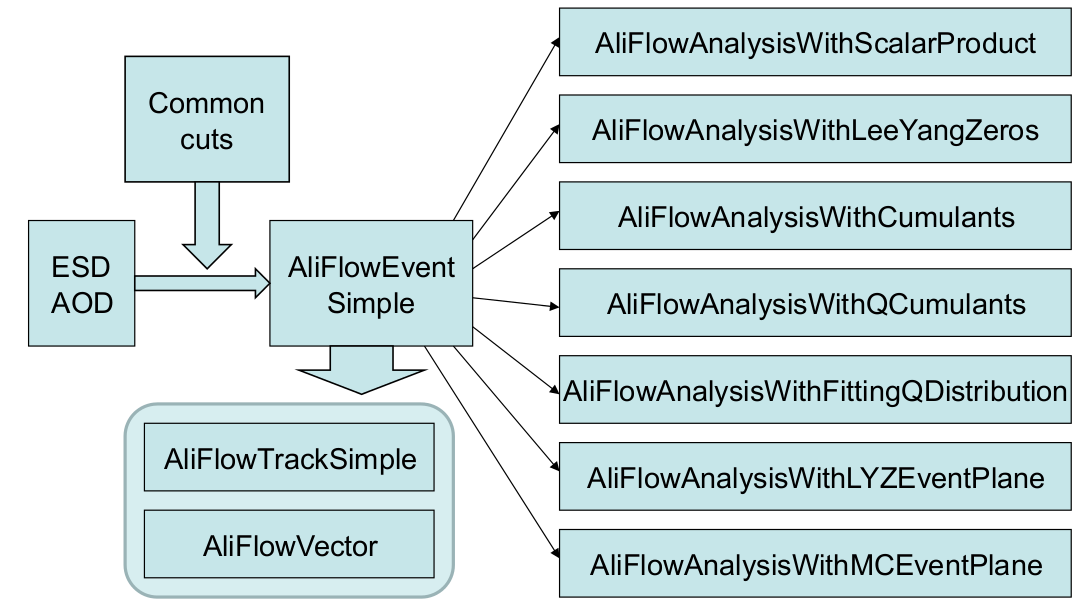
\includegraphics[width=.75\textwidth]{figs/flowChart.png}
\caption{Schematic presentation of the organization of the flow package. Input, which can come from any kind of source, is converted to a generic \texttt{AliFlowEventSimple} object, which in turn is passed to the analysis methods.}
\label{fig:flowchart}
\end{center}
\end{figure}
Figure \ref{fig:flowchart} gives a simple schematic representation of the flow package. Input events (in the case of the figure this is either ESDs or AODs) pass a set of event cuts (the common cuts) and are then converted to a flow event (stored as an \texttt{AliFlowEventSimple} object). This flow event holds a collection of flow tracks (\texttt{AliFlowTrackSimple} objects) which are passed to flow analysis methods. The only steps of this flow chart which depend on \texttt{AliROOT} libraries are the ones handling \textt{ALICE} data types (the ESDs or AODs). The rest of the analysis chain (the \texttt{AliFlowEventSimle} and the analysis methods) have no specific \texttt{AliROOT} dependence and are just simple \texttt{c++} objects. Therefore, the flow package is split into two libraries
\begin{description}
\item [libPWGflowBase] The base library, which has no specific \texttt{AliROOT} dependencies. This library holds objects such as the \texttt{AliFlowEventSimple} and \texttt{AliFlowTrackSimple}, and analysis methods classes. The analysis methods classes follow the naming scheme: \texttt{AliFlowAnalysisWith$\ast$} where $\ast$ denotes a specific analysis method. All classes which end up in the \text{libPWGflowBase.so} shared object can be found in \texttt{\$ALICE\_ROOT/PWG/FLOW/Base};
\item [libPWGflowTasks] The tasks library, which has specific \texttt{AliROOT} dependencies. Contrary to what the name suggests, this library does not just hold tasks, but actually comprises all classes of the flow package which need to include \texttt{AliROOT} specific classes. This ranges from classes to read the AOD or ESD input data (important examples are the \texttt{AliFlowEvent} and \texttt{AliFlowTrackCuts}, which will be discussed later on in this chapter) and the \texttt{AliAnalysisTask$\ast$} classes, which are analysis tasks, derived from \texttt{AliAnalysisTaskSE} which can be used in the \texttt{AliROOT} analysis framework and are actually just interface classes to the underlying flow analysis methods of libPWGflowBase. The \text{libPWGflowTasks.so} shared object can be found in \texttt{\$ALICE\_ROOT/PWG/FLOW/Tasks};
\end{description}


\section{Flow Event}
Every flow analysis in the flow package starts with the flow event. As mentioned earlier, the flow event is a simple container class which holds a collection of flow tracks, which are in turn fed to the flow analysis methods. 
\subsection{Input data}
Before passing the flow event to the flow analysis methods, it needs to be filled with a set of flow tracks. In general, a distinction is made between \emph{reference particles} (or \emph{RP's}), which are particles that are used to build the \textbf{Q} vector(s), and \emph{particles of interest} (or \emph{POI's}), which are the particles of which you'll calculate the differential flow. The flow event and the flow analysis methods are designed to keep track of which flow tracks are POI's, RP's (or even both at the same time), which is important to avoid auto-correlation effects which can distort the $v_n$ measurement. The user of the flow package however is responsible for properly setting up the analysis! 

The flow event can be filled with input from many sources. In the second chapter of this manual, a simple method has been shown where the flow event (the \texttt{AliFlowEventSimple} object) fills itself by generating a set of Monte Carlo tracks by sampling kinematic variables from supplied p.d.f.'s. Using this method is a very effective tool for testing and developing new flow analysis methods (if you generate events with a certain $v_2(p_t)$ and then retrieve the same $v_2(p_t)$ from your flow analysis method, you can use that as a tool to proof the validation of your analysis method) but if you want to do a data analysis, a somewhat more advanced - but not difficult - approach is necessary. 

Filling a flow event from data can be performed either `by-hand' (which is covered in section \ref{sec:exotic} on more exotic analyses), but the most commonly used method of filling a flow event in the \texttt{AliROOT} analysis framework is using the dedicated task \texttt{AliAnalysisTaskFlowEvent}. 



or by using the class \texttt{AliFlowEvent}. \texttt{AliFlowEvent} is a derived class. Its  base class, \texttt{AliFlowEventSimple} 


\section{Track cuts and the track cuts object}
\subsection{ESD tracks as data source}
\subsection{AOD tracks as data source}
\subsection{Additional options}
\subsubsection{Identified particles}
\subsubsection{VZERO}

Calibration specifics - different for 10h and 11h!
\begin{description}
\item [LHC10h]
\begin{itemize}
\item Re-weighting of vzero signal per tile
\item Re-centering of q-vectors
\item Needs aodb 
\end{itemize}
\item [LHC11h]
\begin{itemize}
\item Dedicated VZERO-EP task
\item Q-vectors are read from event header
\item Needs dedicated task
\end{itemize}
\end{description}
Calibration procedure is selected by AliFlowEvent depending on runnumber
\begin{itemize}
\item User is responsible for enabling VZERO-EP task in case of 11h data!
\end{itemize}
See comments at AliFlowTrackCuts::GetStandardVZEROOnlyTrackCuts2011()
\begin{description}
\item [What is re-weighting ?]
\begin{itemize}
\item Take a TProfile with average multiplicity per cell (for each run)
\item Fit a constant line per disc (or ring) $x = a$ (see next slide for example)
\item The track weight for each VZERO cell is now calculated in a second iteration as
\end{itemize}
\begin{equation}
\mbox{track weight} = \frac{\mbox{cell multiplicity} * a}{\mbox{average multiplicity in a cell}} \nonumber
\end{equation}
\item [What is re-centering ?]
\begin{itemize}
\item Store the $Q$-vectors (component-wise) of a run in a TProfile
\item The corrected $Q$-vectors can now be obtained by doing
\begin{equation}
Q_n \longrightarrow \frac{Q_n - \langle Q_n \rangle }{\sigma_{Q_n}} \nonumber
\end{equation}
where brackets denote the one-run average, and $\sigma_{Q_n}$ the standard deviation of $Q_n$ in the sample
\end{itemize}
\end{description}

Several options for VZERO signal calibration in 10h system
\begin{itemize}
\item Per ring re-weighting (instead of full-disc reweighting) \\
\alert{AliFlowTrackCuts::SetV0gainEqualizationPerRing(bool)}
\end{itemize}
\begin{center}
\includegraphics[width=.4\textwidth]{figs/eg_disc.pdf}
\includegraphics[width=.4\textwidth]{figs/eg_ring.pdf}
\end{center}
\begin{itemize}
\item Toggle on or off the additional q-vector recentering \\
AliFlowTrackCuts::SetApplyRecentering(bool)
\item Toggle: disable or enable offending rings from the entire computation (will break re-centering) \\
AliFlowTrackCuts::SetUseVZERORing(int, bool)
\end{itemize}
In 11h, none of these options are available, \alert{everything is done in the VZERO-EP task}!


\section{The flow package in the ALICE analysis framework}
\subsection{AliAnalysisTaskSE}
\subsection{Analysis methods}

\begin{itemize}
\item AliFlowAnalysisWithCumulants.h             
\item AliFlowAnalysisWithMixedHarmonics.h
\item AliFlowAnalysisWithFittingQDistribution.h \item  AliFlowAnalysisWithMultiparticleCorrelations.h
\item AliFlowAnalysisWithLeeYangZeros.h          
\item AliFlowAnalysisWithNestedLoops.h
\item AliFlowAnalysisWithLYZEventPlane.h         
\item AliFlowAnalysisWithQCumulants.h
\item AliFlowAnalysisWithMCEventPlane.h          
\item AliFlowAnalysisWithScalarProduct.h
\end{itemize}


\subsection{Example: $\pi^{\pm}$ $v_2$}\label{sec:example}
As an example of how to do a flow analysis using the flow package within the \texttt{AliROOT} analysis framework, this section will guide you through the process of measuring $\pi^{\pm}$ $v_2$ step-by-step. Generally, doing an analysis in the \texttt{AliROOT} is a two-file process, where one runs a run.C script in \texttt{AliROOT}, which sets up the analysis framework and takes care of the interface to the analysis \texttt{GRID}, and calls an \texttt{AddTask$\ast$.C} macro which in turn creates and configures instances of the relevant analysis tasks. In this example, the distinction will not be so clear, but mentioned in the text. In practice of course, you would copy these steps into macros and launch the macros from the \texttt{AliROOT} command line when doing analysis. We will not run this test on \texttt{GRID}, but assume that you have some \texttt{AliAOD.root} files available on your local system. Note that this example is a guideline, there are many ways leading to Rome, and many ways of setting up an analysis. 

\begin{description}
\item [Preparing the session] First, we need to prepare the framework and root session (these steps would go into your run.C macro). Launch \texttt{AliROOT} and load the necessary libraries
\begin{lstlisting}
  // load libraries
  gSystem->Load("libCore.so");        
  gSystem->Load("libGeom.so");
  gSystem->Load("libVMC.so");
  gSystem->Load("libPhysics.so");
  gSystem->Load("libTree.so");
  gSystem->Load("libSTEERBase.so");
  gSystem->Load("libESD.so");
  gSystem->Load("libAOD.so");
  gSystem->Load("libANALYSIS.so");
  gSystem->Load("libANALYSISalice.so");
  gSystem->Load("libEventMixing.so");
  gSystem->Load("libCORRFW.so");
  gSystem->Load("libPWGTools.so");
  gSystem->Load("libPWGCFebye.so");
  gSystem->Load("libPWGflowBase.so");
  gSystem->Load("libPWGflowTasks.so"); \end{lstlisting}
Create an analysis manager and create a \texttt{TChain} which we will point to the data you have stored locally on your machine
\begin{lstlisting}
  // create the analysis manager
  AliAnalysisManager* mgr = new AliAnalysisManager("MyManager");
  // create a tchain which will point to an aod tree
  TChain* chain = new TChain("aodTree");
  // add a few files to the chain
  chain->Add("/home/rbertens/Documents/CERN/ALICE_DATA/data/2010/LHC10h/000139510/ESDs/pass2/AOD086/0003/AliAOD.root");
  chain->Add("/home/rbertens/Documents/CERN/ALICE_DATA/data/2010/LHC10h/000139510/ESDs/pass2/AOD086/0003/AliAOD.root");
  chain->Add("/home/rbertens/Documents/CERN/ALICE_DATA/data/2010/LHC10h/000139510/ESDs/pass2/AOD086/0004/AliAOD.root");
  chain->Add("/home/rbertens/Documents/CERN/ALICE_DATA/data/2010/LHC10h/000139510/ESDs/pass2/AOD086/0005/AliAOD.root");
  chain->Add("/home/rbertens/Documents/CERN/ALICE_DATA/data/2010/LHC10h/000139510/ESDs/pass2/AOD086/0006/AliAOD.root");
  chain->Add("/home/rbertens/Documents/CERN/ALICE_DATA/data/2010/LHC10h/000139510/ESDs/pass2/AOD086/0007/AliAOD.root");
  chain->Add("/home/rbertens/Documents/CERN/ALICE_DATA/data/2010/LHC10h/000139510/ESDs/pass2/AOD086/0008/AliAOD.root");
  chain->Add("/home/rbertens/Documents/CERN/ALICE_DATA/data/2010/LHC10h/000139510/ESDs/pass2/AOD086/0009/AliAOD.root");
  chain->Add("/home/rbertens/Documents/CERN/ALICE_DATA/data/2010/LHC10h/000139510/ESDs/pass2/AOD086/0010/AliAOD.root");
  // create an input handler
  AliVEventHandler* inputH = new AliAODInputHandler();
  // and connect it to the manager
  mgr->SetInputEventHandler(inputH);\end{lstlisting}
Great, at this point we have created an analysis manager, which will read events from a chain of AliAOD.root files. 
  
The next step will be adding specific analyses to the analysis manager. This is usually done by calling an \texttt{AddTask$\ast$.C} macro, which creates instances of analysis tasks, connects input (events from the analysis manager) to these tasks, and then connects output from the task back to the analysis manager (which will take care of writing the analysis to a common output file). These next steps show what would be in your \texttt{AddTask$\ast$.C} macro.
  
The heart of our flow analysis will be the flow event. To fill a flow event from the input AOD events, we will use the \texttt{AliAnalysisTaskFlowEvent} class. The AOD input events have to be supplied by the analysis manager, so first things first, retrieve the manager to which you will connect your flow analysis tasks:

\begin{lstlisting}
  // the manager is static, so get the existing manager via the static method
  AliAnalysisManager *mgr = AliAnalysisManager::GetAnalysisManager();
  if (!mgr) {
      printf("No analysis manager to connect to!\n");
      return NULL;
  }
        
  // just to see if all went well, check if the input event handler has been connected
  if (!mgr->GetInputEventHandler()) {
      printf("This task requires an input event handler!\n");
      return NULL;
    }\end{lstlisting}
    
The manager and input data are present, so we can create the flow event task and do some basic configuration
\begin{lstlisting}
  // create instance of the class
  AliAnalysisTaskFlowEvent* taskFE = new AliAnalysisTaskFlowEvent("FlowEventTask");
  // enable QA plots (will give you more insight into what you're doing)
  taskFE->SetQAOn(kTRUE);
  // set the trigger selection
  taskFE->SelectCollisionCandidates(AliVEvent::kMB);
\end{lstlisting}
Note that in the last step you have set the trigger configuration. Always make sure that you run on a trigger that makes sense for your analysis. A general remark is that the non-uniform acceptance correction methods that are implemented in the flow package, assume a flat \textbf{Q} vector distribution. Specific triggers (e.g. EMCal triggers) result in a \textbf{Q} vector bias which should \emph{not} be corrected as they invalidate that assumption\footnote{The actual event selection based on triggers is done in the \texttt{AliAnalysisTaskSE} class (to be specific, the trigger is checked in \texttt{AliAnalysisTaskSE::Exec()}) from which the \texttt{AliAnalysisTaskFlowEvent} is derived. The full set of available triggers can be found in the virtual event header \texttt{AliVEvent.h}. }.

In addition to the trigger selection, one might want to do some more event selection. The flow package has a common event selection class, which we will add to your flow event

\begin{lstlisting}
  // define the event cuts object
  AliFlowEventCuts* cutsEvent = new AliFlowEventCuts("EventCuts");
  // configure some event cuts, starting with centrality
  cutsEvent->SetCentralityPercentileRange(20., 30.);
  // method used for centrality determination
  cutsEvent->SetCentralityPercentileMethod(AliFlowEventCuts::kV0);
  // vertex-z cut
  cutsEvent->SetPrimaryVertexZrange(-10.,10.);
  // enable the qa plots
  cutsEvent->SetQA(doQA);
  // explicit multiplicity outlier cut
  cutsEvent->SetCutTPCmultiplicityOutliersAOD(kTRUE);
  cutsEvent->SetLHC10h(kTRUE);
  
  
  // and, last but not least, pass these cuts to your flow event task
  taskFE->SetCutsEvent(cutsEvent);\end{lstlisting}

Now that the flow event task has been created and some basic configuration has been done, it's time to specify the POI and RP selection. This is done by defining sets of track selection criteria for both POI's and RP's: tracks in an event that pass the track selection criteria are used as POI or RP. The track selection is defined in \texttt{AliFlowTrackCuts} objects which are passed to the \texttt{AliAnalysisTaskFlowEvent} task which does the actual selection based on the passed criteria. So, let's create some track selection objects!

Starting with the RP's, for which we'll just use a uniform selection of charged tracks,
\begin{lstlisting}
  //create the track cuts object using a static function of AliFlowTrackCuts
  AliFlowTrackCuts* cutsRP = AliFlowTrackCuts::GetAODTrackCutsForFilterBit(1);
  // specify the pt range
  cutsRP->SetPtRange(0.2, 5.);
  // specify eta range
  cutsRP->SetEtaRange(-0.8, 0.8);
  // specify track type
  cutsRP->SetParamType(kAOD);\end{lstlisting}
  
The particles of which we want to measure the differential $v_2$ are the charted pions. The \texttt{AliFlowTrackCuts} will do the particle identification. 
  
\begin{lstlisting}
  //create the track cuts object using a static function of AliFlowTrackCuts
  AliFlowTrackCuts* cutsPOI = AliFlowTrackCuts::GetAODTrackCutsForFilterBit(1);
  
  // specify the track type
  cutsPOI->SetParamType(kAOD);\end{lstlisting}

\end{lstlisting}
\begin{lstlisting}

\end{lstlisting}
\begin{lstlisting}

\end{lstlisting}
\begin{lstlisting}

\end{lstlisting}
\begin{lstlisting}

\end{lstlisting}
\begin{lstlisting}

\end{lstlisting}
\begin{lstlisting}

\end{lstlisting}
\begin{lstlisting}

\end{lstlisting}
\begin{lstlisting}

\end{lstlisting}
\begin{lstlisting}

\end{lstlisting}
\begin{lstlisting}

\end{lstlisting}
\begin{lstlisting}

\end{lstlisting}
\begin{lstlisting}

\end{lstlisting}
\begin{lstlisting}

\end{lstlisting}
\begin{lstlisting}

\end{lstlisting}
\begin{lstlisting}

\end{lstlisting}



\begin{lstlisting}

\end{lstlisting}


\end{description}

\chapter{Methods}
\label{Methods}
The flow package aims at providing the user with most of the known flow analysis methods. Detailed theoretical overview of the methods can be found in the following papers, which are included in the folder \texttt{\$ALICE\_ROOT/PWGCF/FLOW/Documentation/otherdocs/}
\begin{itemize}
	\item The Monte-Carlo Truth
	\item Scalar Product Method \\ \hspace*{1cm} \texttt{EventPlaneMethod/FlowMethodsPV.pdf}
	\item Generating Function Cumulants \\ \hspace*{1cm} \texttt{GFCumulants/Borghini\_GFCumulants\_PracticalGuide.pdf}
	\item Q-vector Cumulant method \\ \hspace*{1cm} \texttt{QCumulants/QCpaperdraft.pdf} 
        \item Lee-Yang Zero Method \\ \hspace*{1cm} \texttt{LeeYangZeroes/Borghini\_LYZ\_PracticalGuide.pdf}
	\item Lee-Yang Zero Method \\ \hspace*{1cm} \texttt{LeeYangZeroesEP/LYZ\_RP.pdf}
\end{itemize}
The structure of this  chapter is as follows: of each of the available methods a short description is given in the \texttt{theory} subsection (for more detailed information, see the papers listed above) followed by details which are specific to the implementation in the subsection \texttt{implementation}. Caveats, possible issues, etc, are listed in the \texttt{caveats} subsections. 
%-----------------------------------------------------------------------

\section{AliFlowAnalysisWithCumulants}
\subsection{Theory}
\subsection{Implementation}
\begin{lstlisting}

\end{lstlisting}

\section{AliFlowAnalysisWithMixedHarmonics}
\subsection{Theory}
\subsection{Implementation}
\begin{lstlisting}

\end{lstlisting}

\section{AliFlowAnalysisWithFittingQDistribution}
\subsection{Theory}
\subsection{Implementation}
\begin{lstlisting}

\end{lstlisting}


\section{AliFlowAnalysisWithMultiparticleCorrelations}
\subsection{Theory}
\subsection{Implementation}
\begin{lstlisting}

\end{lstlisting}


\section{AliFlowAnalysisWithLeeYangZeros}
\subsection{Theory}
\subsection{Implementation}
\begin{lstlisting}

\end{lstlisting}


\section{AliFlowAnalysisWithNestedLoops}
\subsection{Theory}
\subsection{Implementation}
\begin{lstlisting}

\end{lstlisting}


\section{AliFlowAnalysisWithLYZEventPlane}
\subsection{Theory}
\subsection{Implementation}
\begin{lstlisting}

\end{lstlisting}


\section{AliFlowAnalysisWithQCumulants}

	\label{qvc}
	\subsection{Theory}
	The Q-cumulant (QC) method\footnote{The overview given in this section is inspired by \cite{bilandzic-2011-83}, for further reading the reader is referred there. A full derivation of results that are relevant in this study is given in appendix \ref{qcapp}.} uses multi-particle correlations to estimate $v_n$ estimates for RP's and POI's, but does not limit itself to two-particle correlations. Although higher-order Q-cumulant calculations are available, this section will discuss the method using two- and four-particle correlations. 
		
	%\paragraph{Multiparticle correlations and anisotropic flow}
	Multi-particle correlations in the QC method are expressed in terms of cumulants, which are the the expectation values of correlation terms in joint probability density functions. Consider the following: if two observables $f$ for particles $x_i$ and $x_j$ are correlated, the joint probability $f(x_i, x_j)$ is the sum of the factorization of the constituent probabilities and a covariance term:
	\begin{equation}
		f(x_i, x_j) = f(x_i)f(x_j) + f_c (x_i, x_j)
	\end{equation}
	When taking as an observable azimuthal dependence,
	\begin{align}
		x_i \equiv e^{i n \phi_i}, \hspace{.5in} x_j \equiv e^{i n \phi_j} 
	\end{align}
	the two-particle cumulant is expressed as the covariance of the expectation value:
	\begin{equation}
		E_C(e^{i n[\phi_i - \phi_j]}) = E(e^{[i n(\phi_i - \phi_j]}) - E(e^{in[\phi_i]})E(e^{in[- \phi_j]}).
	\end{equation}
	Symmetry arguments (along the lines of those given in appendix \ref{sec:harmonic_derivation}) dictate that the product of separate expectation values is equals zero, from which a familiar expression for the two-particle correlation is obtained:
	\begin{align}
		E_C(e^{i n[\phi_i - \phi_j]}) & = E(e^{in[\phi_i]})E(e^{in[- \phi_j]})                                   \\
		                              & = \left< e^{in[\phi_i]}\right> \left< e^{in[- \phi_j]} \right> \nonumber \\
		                              & = \left< e^{in[\phi_i - \phi_j]} \right> \nonumber                       \\
		                              & = \left< 2 \right>, \nonumber                                            
	\end{align}
	the all-event average of which is denoted by
	\begin{equation}\label{twocul}
		c_n\{2\} = \left< \left< 2 \right> \right>
	\end{equation}
	where $c_n\{2\}$ is called the two-particle cumulant. For the four-particle case, one proceeds likewise:
	\begin{align}
		E_c(e^{in[\phi_i + \phi_j - \phi_k -\phi_l]}) & = E(e^{in[\phi_i + \phi_j - \phi_k -\phi_l]})                     \\
		                                              & - E(e^{in[\phi_i - \phi_k]})E(e^{in[\phi_j - \phi_l]})\nonumber   \\
		                                              & - E(e^{in[\phi_i - \phi_l]})E(e^{in[\phi_j - \phi_k]}). \nonumber 
	\end{align}
	The four-particle cumulant can be expressed in terms of two- and four-particle correlations as well,
	\begin{equation}\label{fourcul}
		c_n\{4\} = \left< \left< 4 \right> \right> - 2 \left< \left< 2 \right> \right>^2.
	\end{equation}
	From \ref{twocul} and \ref{fourcul} it follows that $v_n$ harmonics are related to cumulants following
	\begin{align}\label{refFlowFromCumulants2nd}
		v_n\{2\} & = \sqrt{c_n\{2\}}                \\
		v_n\{4\} & = \sqrt[4]{-c_n\{4\}} \nonumber. 
	\end{align}
	where $v_n\{2\}$, $v_n\{4\}$ denote flow estimates obtained from two- and four-particle correlations.
		
	In a fashion similar to that explained in the previous subsection, the Q-cumulant method uses reference flow to obtain a statistically stable estimate of the differential flow of POI's. Differential POI flow, for the two- and four-particle case, can be expressed as
	\begin{align}
		d_n\{2\} & = \left< \left< 2^{\prime} \right> \right>                                                                                            \\
		d_n\{4\} & = \left< \left< 4^{\prime} \right> \right> - 2\cdotp \left< \left< 2^{\prime} \right> \right>\left< \left< 2 \right> \right>\nonumber 
	\end{align}
	where $d_n\{2\}, d_n\{4\}$ denotes the two-, four-particle differential flow and the $^{\prime}$ is used as an indicator for differential (p$_t$ dependent) results. Disentangling from this the reference flow contributions, one is left with the final expression for the estimate of differential $v_n$ for POI's:
	\begin{align}
		v_n^{\prime}\{2\} & = \frac{d_n\{2\}}{\sqrt{c_n\{2\}}}               \\
		v_n^{\prime}\{4\} & = - \frac{d_n\{4\}}{(-c_n\{2\})^{3/4}}.\nonumber 
	\end{align}
		
	\subsection{Implementation}
A how-to of the QC method in the flow-package is written by the author of the analysis software and is available on the FLOW-PAG twiki page (\href{https://twiki.cern.ch/twiki/bin/view/ALICE/FlowPackageHowto}{https://twiki.cern.ch/twiki/bin/view/ALICE/FlowPackageHowto}). This section is copied from the twiki page.

 To get the first feeling how the FLOW package and QC output are organized, perhaps you can just trivially execute one 'on-the-fly' example 

 Essentially, you have to do two things: 
	\begin{lstlisting}
cp $ALICE_ROOT/PWGCF/FLOW/macros/runFlowAnalysisOnTheFly.C
aliroot runFlowAnalysisOnTheFly.C \end{lstlisting}

 In the analysis on-the-fly particles are sampled from hardwired Fourier-like p.d.f, so input vn harmonics are completely under control. Please have a look at the steering macro runFlowAnalysisOnTheFly.C and corresponding class AliFlowEventSimpleMakerOnTheFly.cxx in the FLOW package, which are easily written (no fancy C++ features in my code!), and well documented. 

 If you have landed successfully, you will get an output AnalysisResults.root, where the results from each method are structured in directories. 

 To make a size of the file lighter (which matters a lot during merging!), you may want not to use all the methods. You can make your selection of the methods via:
 	\begin{lstlisting}
Bool_t MCEP = kTRUE; // Monte Carlo Event Plane
Bool_t SP = kTRUE; // Scalar Product (a.k.a 'flow analysis with eta gaps')
Bool_t GFC = kTRUE; // Generating Function Cumulants
Bool_t QC = kTRUE; // Q-cumulants
Bool_t FQD = kTRUE; // Fitted q-distribution
Bool_t LYZ1SUM = kTRUE; // Lee-Yang Zero (sum generating function), first pass over the data
Bool_t LYZ1PROD = kTRUE; // Lee-Yang Zero (product generating function), first pass over the data
Bool_t LYZ2SUM = kFALSE; // Lee-Yang Zero (sum generating function), second pass over the data
Bool_t LYZ2PROD = kFALSE; // Lee-Yang Zero (product generating function), second pass over the data
Bool_t LYZEP = kFALSE; // Lee-Yang Zero Event Plane
Bool_t MH = kFALSE; // Mixed Harmonics (used for strong parity violation studies) 
Bool_t NL = kFALSE; // Nested Loops (neeed for debugging, only for developers) 	\end{lstlisting}
 Next important remark, if you want to browse through AnalysisResults.root, make sure that in AliROOT prompt you have loaded the FLOW library:
 	\begin{lstlisting}
root [0] gSystem->Load("libPWGflowBase"); 	\end{lstlisting}
 In the AnalysisResults.root, the QC output is stored in "outputQCanalysis". Just browse there, browse in "cobjQC", and you will see the directory structure.
 "Integrated Flow" => contains all results needed for reference flow. Browse in, and explore the directory (in fact, TList) "Results". The names of the histos should be self-explanatory;
 "Differential Flow" => browse further into "Results", and you will find a bunch of things that you can explore. For instance, in the directory "Differential Q-cumulants (POI,p$_{T}$)" you will find histos holding differential QC\{2\} vs pt, QC\{4\} vs p$_{T}$, etc. On the other hand, the flow estimates themselves, namely differential vn\{2\} vs pt, vn\{4\} vs pt you can fetch from TList "Differential Flow (POI,p$_{T}$)"
 I hope that the names for all other things you might need are self-explanatory. 
 You configure QC method in the steering macro via setters:
 	\begin{lstlisting}
qc->SetHarmonic(2);
qc->SetCalculateDiffFlow(kTRUE);
qc->SetCalculate2DDiffFlow(kFALSE); // vs (pt,eta)
qc->SetApplyCorrectionForNUA(kFALSE);
qc->SetFillMultipleControlHistograms(kFALSE); 
qc->SetMultiplicityWeight("combinations"); // default (other supported options are "unit" and "multiplicity")
qc->SetCalculateCumulantsVsM(kFALSE);
qc->SetCalculateAllCorrelationsVsM(kFALSE); // calculate all correlations in mixed harmonics "vs M"
qc->SetnBinsMult(10000);
qc->SetMinMult(0);
qc->SetMaxMult(10000); 
qc->SetBookOnlyBasicCCH(kFALSE); // book only basic common control histograms
qc->SetCalculateDiffFlowVsEta(kTRUE); // if you set kFALSE only differential flow vs pt is calculated
qc->SetCalculateMixedHarmonics(kFALSE); // calculate all multi-partice mixed-harmonics correlators	\end{lstlisting}
 You can make QC output lighter by setting 
 	\begin{lstlisting}
qc->SetBookOnlyBasicCCH(kTRUE);	\end{lstlisting} 
(to book only basic control histograms, and disabling lot of 2D beasts), and 
	\begin{lstlisting}
qc->SetCalculateDiffFlowVsEta(kFALSE); 	\end{lstlisting}
(if not interested in differential flow vs eta => this will make the final output smaller) 
 In the "cobjQC" you might also consider "AliFlowCommonHistQC" to be useful thing, which contains a lot of trivial but still important control histograms (eg multiplicity distribution of RPs, POIs, etc). 
 I think this is the best and fastest way for you to get familiar with the FLOW package => once you send the QC code over the real data, you get the output organized in the very same way. I will send you shortly an example set of macros which get be used for the analysis on Grid over the real data. 
 Differential QC\{2\} and QC\{4\} implementation is generic. You can tag as RP and POI whatever you want, and it will give you results automatically decoupled from any autocorrelation effects. For this reason, it is important that if you have certain particles which is classified both as RP and POI, to be explicitly tagged also as RPs and POI once you are building the "flow event". 
 The basic feature in the FLOW package is that from whichever input you start, we have to build the same intermediate step called "flow event", with which than we feed all methods (SP, QC, etc) in the very same way. 
 To see what "flow event" does, and what does it need as an input, you may want to consult task AliAnalysisTaskFlowEvent.cxx and classes needed there-in. 



\section{AliFlowAnalysisWithMCEventPlane}
\subsection{Theory}
\subsection{Implementation}
\begin{lstlisting}

\end{lstlisting}



\section{AliFlowAnalysisWithScalarProduct}
\label{SP}
\subsection{Theory}
\subsubsection{The scalar product method}
The scalar product method - as well as the Q-cumulant method which will be described later - does not depend on explicit construction of an (sub)event plane, but estimates $v_n$ directly from multi-particle correlations. 

To do so, firstly all particles in an event are labeled either as \emph{reference particles} (RP's) or \emph{particles of interest} (POI's). The RP and POI selections are in turn divided into sub-events, which are again taken from different $\eta$ ranges, in analogy to the approach taken for the event plane method. Each POI is correlated with a sub-event Q-vector from the RP selection, which allows for the calculation of $v_n$ without any explicit reconstruction of an event plane\cite{sp}. 

The reason for the division into RP's and POI's is the fact that the two particle correlator of POI's,
\begin{equation}\label{unstable}
	v_n^{POI} = \sqrt{ \left< e^{i n (\phi^{POI}_i - \phi^{POI}_j)} \right> }
\end{equation}
is generally not stable statistically. Introducing reference flow, \ref{unstable} can be rewritten as
\begin{equation}\label{stable}
	v_n^{POI} = \frac{ \left< e^{i n (\phi^{POI}_i - \phi^{RP}_j)} \right>}{\left< e^{i n (\phi^{RP}_i - \phi^{RP}_j)} \right>} = \frac{v_n^{POI} v_n^{RP} }{\sqrt{v_n^{RP} v_n^{RP}}}.
\end{equation}
By taking an abundant particle source as RP's - in the case of this study the RP selection comprises all charged particles - both correlators in \ref{stable} are statistically stable. 

\paragraph{The scalar product method}
In the scalar product method, POI's $u_k$,
\begin{equation}\label{spderiv}
	u_k = e^{i n \phi_k},
\end{equation}
are correlated with $Q^*_a$, the complex-conjugate Q-vector built from RP's in a given sub-event $a$. First, the scalar product of $u_k$ and $Q^*_a$ is taken,
\begin{equation}
	u_k \cdotp \sum_{\substack{ j=1,\\j \neq k}}^{M_{RP, a}} u^*_j
\end{equation}
where $M_{RP, a}$ denotes RP multiplicity for a given sub-event $a$ and the inequality $j \neq k$ removes auto-correlations. From this, differential $v_n$ of POI's ($v_n^{\prime}$) and $v_n$ of RP's ($v_n^a$) in sub-event $a$ can be obtained in a straightforward way from the correlation of POI's and RP's:
\begin{equation}\label{rppoisp}
	\left< u \cdotp Q^*_a \right> = \frac{1}{M_{RP, a}-k}\sum_{i=k}^{M_{RP, a}} \left( u_k \sum_{\substack{ j=1,\\j \neq k}}^{M_{RP, a}} u^*_j \right)
\end{equation}
where POI multiplicity is expressed in terms of $M_{RP, a}$; $M_{POI} = M_{RP, a} - k$. Since for any function $f(x)$ and constant $a$
\begin{equation}
	\sum a f(x) = a \sum f(x) 
\end{equation}
\ref{rppoisp} can be rewritten as
\begin{align}\label{sp_part2}
	\left< u \cdotp Q^*_a \right> & = \frac{1}{M_{RP, a}-k}\sum_{i=k}^{M_{RP, a}} e^{i n [\phi_k - \Psi_n]} \sum_{j=1}^{M_{RP, a}} e^{- i n [\phi_j - \Psi_n]} \\
	                              & = M_{RP, a} v^{\prime}_n v_n^a \nonumber                                                                                   
\end{align}
where in the last step of \ref{sp_part2} it has been used that
\begin{equation}
	v_n = \frac{\ds \sum_i^M e^{in[\phi_i - \Psi_n]} }{M}.
\end{equation}

To obtain the estimate of $v_n$, one must still disentangle the reference flow contribution from the event averaged correlation given in \ref{rppoisp}. 
Proceeding in a fashion similar to that presented in equation \ref{rppoisp}, it can be shown that
\begin{equation}
	\left< \frac{Q_a}{M_a}\cdotp\frac{Q^*_b}{M_b} \right> = \left< v_n^{a}v_n^{b} \right>
\end{equation}
where $Q_a, Q_b$ are the Q-vectors of RP's in sub-event $a, b$. Under the assumption that
\begin{equation}\label{zerononflow}
	\left< v_n^2 \right> = \left< v_n \right>^2,
\end{equation}
- an assumption which will be spoiled in the case of flow fluctuations - and requiring that the $v_n$ estimates in both sub-events are equal, one simply evaluates
\begin{equation}\label{sp}
	v_n^{\prime} = \frac{\left< \left< u \cdotp \frac{Q^*_a}{M_a} \right>\right>}{\sqrt{ \left< \frac{Q_a}{M_a}\cdotp\frac{Q^*_b}{M_b} \right>}}
\end{equation}
to obtain $v_n^{a}$. For equal multiplicity sub-events $M_a = M_b$, \ref{sp} is simplified to
\begin{equation}\label{spa}
	v_n^{\prime} = \frac{\left< \left< u \cdotp Q^*_a \right>_t \right>}{ \sqrt{ \left< Q_a\cdotp Q^*_b \right>}}.
\end{equation}
$v_n^b$ can be obtained by switching indices $a$ and $b$ in expressions \ref{sp} and \ref{spa}, and should equal $v_n^a$.
This principle can be generalized straightforwardly to allow for a selection of RP's which has been divided into three subevents. 
\begin{align}
	v_n^a & = \frac{ \left< \left< u \cdotp \frac{Q^*_a}{M_a} \right> \right>}{\sqrt{\left< v_n^{\prime a} v_n^{\prime b} \right> \left< v_n^{\prime a}v_n^{\prime c} \right> / \left< v_n^{\prime b} v_n^{\prime c} \right>}}                                                    \\
	      & = \frac{\left< \left< u \cdotp \frac{Q^*_a}{M_a} \right> \right>}{\sqrt{\left< \frac{Q_a}{M_a} \cdotp \frac{Q_{b}^{*}}{M_b} \right> \left< \frac{Q_a}{M_a} \cdotp \frac{Q_{c}^{*}}{M_c} \right> / \left< \frac{Q_b}{M_b} \cdotp \frac{Q_c^*}{M_c}} \right>} \nonumber 
\end{align}
where cyclic permutation of $a, b, c$ (in analogy to the switching of indices in \ref{3evsp} gives the estimates of $v_n^b$ and $v_n^c$.\textcolor{red}{[insert some discussion here: is this result actually true, and some light on va, vb, (vc)]}

\subsubsection{Extension to Event Plane method}
As explained earlier, the event plane analysis results in this study are actually obtained by normalizing the Q-vectors in the scalar product by their length $\vert Q_n \vert$. Consider the following:
\begin{equation}\label{phase}
	\frac{Q_n^*}{\vert Q_n^* \vert} = \frac{\vert Q_n^* \vert e^{- i n \Psi_{Q_n}}}{\vert Q_n^* \vert} = e^{- i n \Psi_{Q_n}}.
\end{equation}
For a full event, the enumerator of \ref{sp} can be expressed as
\begin{equation}\label{epsp1}
	\left< \left< u \cdotp e^{- i n \Psi_{Q_n}} \right> \right> = \left< \left< e^{i n \phi_i} \cdotp e^{- i n \Psi_{Q_n}} \right> \right> \nonumber = \left< \left< e^{i n (\phi_i - \Psi_{Q_n})} \right> \right> = \left< \left< \cos(n [\phi_i - \Psi_{Q_n}]) \right> \right>
\end{equation}
which corresponds to the all-event average of \ref{ep_first}. As shown in the previous subsection this expression equals $v_n^{obs}$. 

For normalized Q-vectors, the denominator of \ref{sp} reads (using \ref{phase}):
\begin{equation}\label{epsp2}
	\sqrt{\left< \frac{Q_a}{\vert Q_a\vert} \cdotp \frac{Q_b^*}{\vert Q_b^* \vert \right>}} = \sqrt{\left< e^{in[\Psi_{Q_{n_a}} - \Psi_{Q_{n_b}}}\right>} = \sqrt{\left< \cos(n[\Psi_{Q_{n_a}} - \Psi_{Q_{n_b}}]\right>)}
	\end{equation}
	from which the event plane resolution can be calculated using \ref{emeancos} or \ref{halfeventresolution}.

\subsection{Implementation}
\begin{lstlisting}
   void SetHarmonic(Int_t iHarmonic)          { fHarmonic = iHarmonic; }
   void SetApplyCorrectionForNUA(Bool_t iVal) { fApplyCorrectionForNUA = iVal?1:0; }
   void SetNormalizationType(Int_t iVal)      { fNormalizationType = iVal; }
   void SetDebug(Bool_t bVal)                 { fDebug = bVal; }
   void SetBookOnlyBasicCCH(Bool_t bVal)           { fMinimalBook = bVal; }
   void SetTotalQvector(Int_t iVal)           { fTotalQvector = iVal; }
   void SetUsePhiWeights(Bool_t bVal)        { fUsePhiWeights = bVal; }
   void SetWeightsList(TList* const aWeightsList)  { fWeightsList = (TList*)aWeightsList->Clone(); }\end{lstlisting}

		\subsubsection{VZERO scalar product}
		
The VZEROA and VZEROC detectors have different $\eta$ coverage w.r.t the TPC, so to evaluate $v_2$ from VZERO-SP, do
\begin{equation}
v_n = \sqrt{\frac{\langle u_i \cdotp Q_A \rangle }{\sqrt{\langle Q_A \cdotp Q_B \rangle}} \cdotp \frac{\langle u_j \cdotp Q_B \rangle }{\sqrt{\langle Q_A \cdotp Q_B \rangle}}}
\nonumber
\end{equation}
\begin{itemize}
\item $Q_A$ and $Q_B$ are the VZEROC and VZEROA RP's
\end{itemize}
There has been some disscussion ...
\begin{itemize}
\item Take $u$ = full TPC = $u_j$ = $u_i$, or do $u_j$ = $\eta < 0$, $u_i$ = $\eta > 0$ ?
\end{itemize}
We should have a common approach to ensure uniform analyses and physics message!
Majority vote has yielded the following:
\begin{itemize}
\item $u$ = full TPC = $u_j$ = $u_i$
\end{itemize}
\begin{equation}
v_n = \sqrt{\frac{\langle u \cdotp Q_A \rangle }{\sqrt{\langle Q_A \cdotp Q_B \rangle}} \cdotp \frac{\langle u \cdotp Q_B \rangle }{\sqrt{\langle Q_A \cdotp Q_B \rangle}}}
\nonumber
\end{equation}
This means we should think about the \alert{correlation} between terms in this equation!
	\subsubsection{Caveats}
		
		
\chapter{More exotic uses}\ref{sec:exotic}
\section{Flow analysis of resonances}	


Reconstructing decayed particles
%\item Invariant mass reconstruction, e.g.
\begin{equation}
\boxed{ \mbox{\Lambda} \longrightarrow \pi + \mbox{p} } \nonumber
\end{equation}
\begin{itemize}
\item Take all the $\pi + \mbox{p}$ pairs in an event and plot their invariant mass
\item Extract the signal yield \alert{$N^S$} and total yield \alert{$N^T$} from this distribution
\item Measure $v_2$ of all $\pi + \mbox{p}$ pairs
\end{itemize}
Under the assumption that signal and background flow are additive, we can disentangle the two
\begin{align}
v_2^{T}(m_{inv})  = & \alert{v_2^{S}} \frac{N^{S} }{N^{S} + N^{B}}(m_{inv}) \nonumber \\ 
& + v_2^{B}(m_{inv}) \frac{ N^{B}}{N^{S} + N^{B}}(m_{inv})\nonumber 
\end{align}
\column{.5\textwidth}
\includegraphics[width=.9\textwidth]{figs/2012-Jul-25-oneOFtwo_16_18.pdf}\\
\includegraphics[width=.9\textwidth]{figs/2012-Jul-25-twoOFtwo_16_18.pdf}
\end{columns}
\end{frame}
	
\section{Flow analysis in the LEGO framework: re-tagging your POI and RP selections}
\subsection{The problem at hand}
\subsection{Re-tagging POI and RP selections}
		
	\chapter{Summary}
	\label{Summary}
	This sums it all up.
	%-----------------------------------------------------------------------
		
	\begin{thebibliography}{99}
				
				  
		\bibitem{Ollitrault:1992bk}
		J.~Y.~Ollitrault,
		%``Anisotropy as a signature of transverse collective flow,''
		Phys.\ Rev.\ D {\bf 46} (1992) 229.
		%%CITATION = PHRVA,D46,229;%%
				
		\bibitem{Danielewicz:1999vh}
		P.~Danielewicz,
		%``Flow and equation of state in heavy-ion collisions,''
		Nucl.\ Phys.\ A {\bf 661} (1999) 82.
		%  [arXiv:nucl-th/9907098].
		%%CITATION = NUCL-TH 9907098;%%
				
		\bibitem{Rischke:1996nq}
		D.~H.~Rischke,
		%``Hydrodynamics and collective behavior in relativistic nuclear
		%collisions,''
		Nucl.\ Phys.\ A {\bf 610} (1996) 88C.
		%  [arXiv:nucl-th/9608024].
		%%CITATION = NUCL-TH 9608024;%%
				
		\bibitem{Ollitrault:1997vz}
		J.~Y.~Ollitrault,
		%``Flow systematics from SIS to SPS energies,''
		Nucl.\ Phys.\ A {\bf 638} (1998) 195.
		%  [arXiv:nucl-ex/9802005].
		%%CITATION = NUCL-EX 9802005;%%
				
		\bibitem{Voloshin:1994mz}
		S.~Voloshin and Y.~Zhang,
		%``Flow study in relativistic nuclear collisions by Fourier expansion of
		%Azimuthal particle distributions,''
		Z.\ Phys.\ C {\bf 70} (1996) 665.
		%  [arXiv:hep-ph/9407282].
		%%CITATION = HEP-PH 9407282;%%
				
		%\cite{Ackermann:2000tr}
		\bibitem{Ackermann:2000tr}  
		K.~H.~Ackermann {\it et al.}  [STAR Collaboration],
		%``Elliptic flow in Au + Au collisions at s(N N)**(1/2) = 130-GeV,''
		Phys.\ Rev.\ Lett.\  {\bf 86} (2001) 402
		%[arXiv:nucl-ex/0009011].  
		%%CITATION = NUCL-EX 0009011;%%
				  
		%\cite{Adler:2001nb}
		\bibitem{Adler:2001nb}  
		C.~Adler {\it et al.}  [STAR Collaboration],
		% ``Identified particle elliptic flow in Au + Au collisions at  
		%s(NN)**(1/2) =  130-GeV,''
		Phys.\ Rev.\ Lett.\  {\bf 87} (2001) 182301  
		%[arXiv:nucl-ex/0107003].  
		%%CITATION = NUCL-EX 0107003;%%
				
		%%% theory RHIC discoveries %%%
		%\cite{Gyulassy:2004zy}
		\bibitem{RHIC_Discoveries}
		T.D.~Lee {\it et al.}, 
		New Discoveries at RHIC: Case for the Strongly Interacting 
		Quark-Gluon Plasma. 
		Contributions from the RBRC Workshop held May 14-15, 2004.
		Nucl.\ Phys.\ A {\bf 750} (2005) 1-171
		%%% end theory white-papers
				
				    
	\end{thebibliography}
		
	%-----------------------------------------------------------------------
%	\chapter*{Appendix I}
%	\label{appendix1}
%	Here we put short pieces of code.
	%-----------------------------------------------------------------------
	\printindex
\end{document}
